\documentclass[10pt, a4paper]{report}

\usepackage[utf8]{inputenc}
\usepackage{polski}
\usepackage{a4wide}
\usepackage{fancyhdr}
\usepackage{lastpage}
\usepackage{tabularx}
\usepackage{graphicx}
\usepackage{listings}
\usepackage{forest}

\graphicspath{ {./images} }

\begin{titlepage}
    \title{\huge{\textbf{Sprawozdanie} \\ programu grapher}}
    \author{Szymon Półtorak i Sebastian Sikorski}
    \date{14.04.2022r}
\end{titlepage}

\renewcommand{\footrulewidth}{1pt}

\begin{document}
    \maketitle

    \renewcommand*\thesection{\arabic{section}}
    
    \begin{abstract}
        Niniejszy dokument jest sprawozdaniem z prac projektowych w ramach projektu \textit{grapher} w języku C.
        W dokumencie został przypomniany cel projektu, opisana struktura folderów, diagram modułów, przedstawione
        wywołania programu wraz z ich wynikami. Podsumowaliśmy projekt oraz współpracę i wysnuliśmy wnioski na temat tego przedsięwzięcia.
    \end{abstract}

    \pagestyle{fancy}
    \fancyhf{}
    \lhead{Sprawozdanie programu \textit{grapher}(C)}
    \rhead{Szymon Półtorak i Sebastian Sikorski}
    \cfoot{Strona \thepage \hspace{1pt} z \pageref{LastPage}}
    
    \fancypagestyle{plain}{
        \lhead{Sprawozdanie programu \textit{grapher}(C)}
        \rhead{Szymon Półtorak i Sebastian Sikorski}
        \cfoot{Strona \thepage \hspace{1pt} z \pageref{LastPage}}
    }
    \tableofcontents
    \newpage

    \section{Cel projektu - streszczenie}
    Program \textit{grapher} ma za zadanie generować pliki z grafami, typu \textit{karta w kratkę}, o z góry ustalonym formacie oraz czytanie takich plików w celu znalezienia najkrótszej ścieżki między zadanymi
    przez użytkownika punktami. Grapher posiada cztery tryby:
    \begin{itemize}
        \item Wage Mode – program generuje graf spójny o losowych wagach krawędzi,
        \item Edge Mode – program losuje istnienie krawędzi między wierzchołkami grafu oraz wagi do
        momentu powstania grafu spójnego,
        \item Random Mode – program losuje istnienie krawędzi i ich wagi. W tym trybie graf może być niespójny,
        \item Read Mode – program czyta plik o ustalonym formacie i szuka najkrótszej ścieżki pomiędzy podanymi przez użytkownika punktami.        
    \end{itemize}
    Po szczegółowe wyjaśnienie funkcjonalności trybów, formatu pliku z grafem oraz znaczenia poszczególnych elementów składni programu odsyłamy do specyfikacji funkcjonalnej projektu \textit{grapher}.

    \section{Struktura programu}
    Program \textit{grapher} skłąda się z 4 folderów nadrzędnych zawierających jego poszczególne elementu. Folder \textit{dokumentacja} zawiera dokumenty opisujące projekt, czyli:
    specyfikację funkcjonalną i implementacyjną oraz końcowe sprawozdania z projektu. Są w nich pliki \textit{*.pdf}, zdjęcia w formacie \textit{*.png} i \textit{*.jpg} oraz kod źródłowy tych dokumnetów w formacie
    \textit{*.tex}. Folder \textit{tests} zawiera kod odpowiedziany za przeprowadzanie testów programu, natomiast folder \textit{src} zawiera pliki z kodem źródłowym oraz pliki nagłówkowe
    programu \textit{grapher}.

    \subsection{Struktura folderów}
    \begin{forest}
        for tree={
          grow'=0,
          child anchor=west,
          parent anchor=south,
          anchor=west,
          calign=first,
          edge path={
            \noexpand\path [draw, \forestoption{edge}]
            (!u.south west) +(7.5pt,0) |- node[fill,inner sep=1.25pt] {} (.child anchor)\forestoption{edge label};
          },
          before typesetting nodes={
            if n=1
              {insert before={[,phantom]}}
              {}
          },
          fit=band,
          before computing xy={l=15pt},
        }
        [\texttt{Grapher}
            [\texttt{dokumentacja}
                [\texttt{Specyfikacja Implementacyjna}
                    [\texttt{images}]
                ]
                [\texttt{Specyfikacja Funkcjonalna}
                ]
                [\texttt{Sprawozdanie}
                    [\texttt{images}]
                ]
            ]
            [\texttt{tests}
            ]
            [\texttt{src}
            ]
            [\texttt{makefile}
            ]
        ]
    \end{forest}
    \newpage

    \subsection{Diagram modułów}
    Projekt \textit{grapher} składa się z modułów: \textit{alloc}, \textit{readGraph}, \textit{genGraph} oraz \textit{utils}. 
    Każdy moduł składa się z pliku nagłówkowego \textit{*.h} oraz pliku z kodem źródłowym \textit{*.c}.
    Posiada on również główny moduł \textit{main} sterujący działaniem całego programu i składa się on tylko z pliku źródłowego \textit{main.c}.
    \begin{figure}[h]
        \begin{center}
            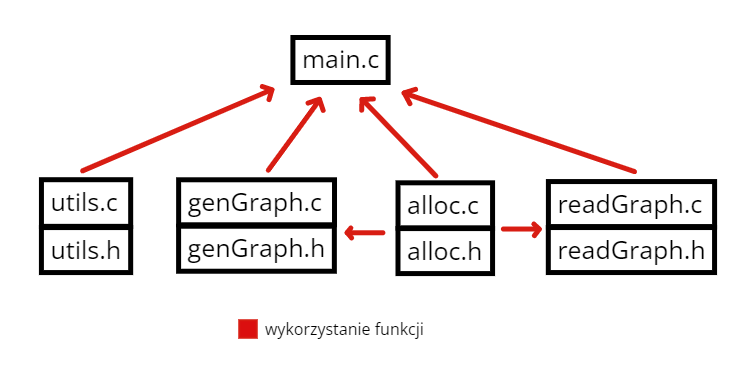
\includegraphics[scale=0.6]{module_diagram_new.png}
            \caption {Diagram modułów}
        \end{center}
    \end{figure}

    \section{Kompilacja programu}
    Program trzeba najpierw skompilować w katalogu głównym projektu. Poniżej przedstawiamy wszystkie komendy możliwe do użycia:
    \begin{itemize}
        \item \texttt{make} - podstawowa kompilacja programu grapher,
        \item \texttt{make clean} - usuwa z programu wszystkie pliki robocze oraz skompilowany plik do uruchamiania programu \textit{grapher},
        \item \texttt{make wm} - kompiluje program i uruchamia go w trybie \textit{wage mode} z góry zakładanymi danymi,
        \item \texttt{make rem} - robi to samo co powyższa komenda ale uruchamia program w trybie \textit{random mode},
        \item \texttt{make em} - wykonuje to samo co powyższe 2 instrukcje ale uruchamia program w trybie \textit{edge mode},
        \item \texttt{make rm} - również wykonuje to samo zadanie ale program korzysta z trybu \textit{read mode}.
    \end{itemize}

    \newpage
    \section{Przykładowe wywołania i wyniki programu}
    W tym rozdziale przedstawimy wywołania programu wraz z ich wynikami dla różnych scenariuszów aby ukazać jak nasz program działa.

    \subsection{Wage Mode}
    \textbf{Plik wejściowy} - w trybach generujących jest to plik pusty.
    \newline Wywołanie:
    \newline\newline \texttt{./grapher -wm -rows 4 -start 1 -file wg.test -end 10 -columns 5}
    \newline\newline Wynik:

    \subsection{Edge Mode}
    \textbf{Plik wejściowy} - plik pusty.
    \newline Wywołanie:
    \newline\newline \texttt{./grapher -em -rows 5 -file em.test -end 20 -columns 7 -start 5}
    \newline\newline Wynik:    

    \subsection{Random Mode}
    \textbf{Plik wejściowy} - plik pusty.
    \newline Wywołanie:
    \newline\newline \texttt{./grapher -file rem.test -rem -end 10 -rows 6 -start 1 -columns 7}
    \newline\newline Wynik:

    \subsection{Read Mode z flagą Standard}
    \textbf{Plik wejściowy} :
    \newline Wywołanie:
    \newline\newline \texttt{./grapher -file rm\_s.test -rm -points 1,5,4,8 -standard }
    \newline\newline Wynik:

    \subsection{Read Mode z flagą Extended}
    \textbf{Plik wejściowy} :
    \newline Wywołanie:
    \newline\newline \texttt{./grapher -extended -points 2,7,3,11 -file rm\_e.test -rm}
    \newline\newline Wynik:

    \section{Zmiany względem specyfikacji}
    W nieniejszym rozdziale opisujemy zmiany jakie zaszły między specyfikacją funkcjonalną i implementacyjną, a wersją finalną programu.

    \subsection{Diagram modułów}
    Z powodu potrzeby dodania nowego modułu zmienił się również diagram modułów. Poprawną wersję prezentowaliśmy już wyżej.
    Doszedł moduł \textit{utils} wspomagający pracę \textit{maina} w zakresie obsługi błędów.

    \subsection{Obsługiwane błędy}
    W trakcie pisania programu napotkaliśmy na sytuacje, które wymagają zdefiniowania nowych błędów żeby użytkownik wiedział, dlaczego program się wyłączył.
    Niestety okazało się również, że nasze kody błędów były zbyt duże i program nie mógł zwracać takich wartości dlatego musieliśmy podjąć decyzję o ich zmianie.
    \newline Poniższa tabela zawiera wszystkie zadeklarowane błędy w programie:
    \newline
    \begin{tabularx}{\textwidth}{ l|c|X } 
        \hline Nazwa Błędu & Kod & Wyjaśnienie błędu\\ 
        \hline NO\_MODE\_FOUND & 230 & Niepoprawny tryb lub jego brak\\ 
        \hline NO\_FILE\_FOUND & 231 & Nie podano pliku lub plik nie istnieje\\ 
        \hline WRONG\_NUM\_OF\_ROWS & 232 & Podano niepoprawną liczbę wierszy\\
        \hline WRONG\_NUM\_OF\_COL & 233 & Podano niepoprawną liczbę kolumn\\
        \hline WRONG\_RANGE\_OF\_WAGES & 234 & Zły zakres losowania wartości wag\\
        \hline NO\_FLAG\_FOUND & 235 & Nie podany flagi w trybie Read Mode\\
        \hline WRONG\_POINTS & 228 & Podano nieistniejący punkt lub ich złą liczbę\\
        \hline NO\_COHERENT & 237 & Graf jest niespójny \\
        \hline NULL\_POINTER\_EXCEPTION & 228 & Alokacja pamięci się nie udała\\
        \hline NOT\_READ\_MODE & 229 & Użyto flagi w trybie do generacji, ale działającej tylko w Read Mode\\
        \hline MULTIPILE\_MODE\_DECLARATION & 230 & Dokonano próby nadpisania zadeklarowanego wcześniej trybu programu\\
        \hline WRONG\_MODE & 227 & Użyto flagi w trybie Read, ale działającej tylko w trybach generujących\\
        \hline
    \end{tabularx}

    \subsection{Zmiany w strukturach}
    Struktury również przeszły małe modyfikacje spowodowane nieprzewidzianymi potrzebami. Zaprezentujemy je poniżej.
    \begin{itemize}
        \item \texttt{struct entryRead} - ta struktura otrzymała nową zmienną \textit{numberPoints} odpowiedzialną za przetrzymywanie liczby
        wszystkich punktów podanych przez użytkownika,
        \begin{lstlisting}
typedef struct entryRead {
    char* fileName;
    bool printFlag;
    int* points;
    int numberPoints;
} entryR;
        \end{lstlisting}
        \item \texttt{struct graphRead} - teraz \textit{graph} jest typu \texttt{node*},
        \begin{lstlisting}
typedef struct graphRead {
    node* graph;
    int rows;
    int columns;
} graphR;
        \end{lstlisting}
        \item \texttt{struct node} - ta struktura otrzymała nową zmienną tablicową \textit{nodeToConnect} oraz wszystkie tablice zostały zmienione ze wskaźników na tablice o określonym rozmiarze. 
        \begin{lstlisting}
typedef struct node {
    bool edgeExist[4]; 
    double edgeWeight[4]; 
    int nodeToConnect[4];
} node;
        \end{lstlisting}        
    \end{itemize}

    \subsection{Wywoływanie programu}
    Zmianom uległo samo wywołanie programu. Poprzednio zakładaliśmy, że użytkownik będzie musiał przestrzegać kolejności wywołania, ale w czasie
    pisania programu stwierdziliśmy, że jest to zadanie bezsensowne i teraz użytkownik może wprowadzać przy pomocy odpowiednich flag w dowolnej kolejności.
    Teraz flagi wymagają od użytkownika podania liczb po niektórych flagach. Poniżej przedstawiamy składnię programu.
    \newline Dla trybów, które generują graf:
    \newline\newline \texttt{./grapher [tryb] [plik] [wiersze] [kolumny] [początek] [koniec]}
    \newline\newline Dla trybu Read mode:
    \newline\newline \texttt{./grapher [tryb] [plik] [flaga] [punkty]}
    \newline\newline Argumenty wymagające podania wartości:
    \begin{itemize}
        \item plik
        \item wiersze
        \item kolumny
        \item początek
        \item koniec
        \item punkty
    \end{itemize}
    Ważnym odnotowania faktem jest to, że punkty powinny zostawać podawane po przecinku przykładowo:
    \newline\newline np.
    \newline \texttt{./grapher -points 1,2,3,4}
    \newline\newline Poniżej w tabeli pokazujemy jak wyglądają wszystkie flagi wraz z ich, krótszymi wersjami jednoliterowymi oraz z krótkim opisem ich działania.
    \newline
    \begin{tabularx}{\textwidth}{ c|c|X }
        \hline Flaga & Literkowy odpowiednik & Funkcja flagi \\
        \hline -points & -p & Służy do określenia punktów w trybie Read Mode.\\
        \hline -file & -f & Służy do załączania pliku, do którego zapisujemy graf lub, z którego czytamy graf.\\
        \hline -rows & -o & Służy do określania liczby wierszy w trybach generujących.\\
        \hline -columns & -c & Służy do wprowadzenia liczby kolumn w trybach generujących.\\
        \hline -start & -t & Pozwala określić początek przedziału losowania wag.\\
        \hline -end & -n & Służy do wprowadzania końca przedziału losowania wag.\\
        \hline -WM & -w & Ustawia tryb działania programu na Wage Mode.\\
        \hline -RM & -r & Ustawia tryb działania programu na Read Mode.\\
        \hline -ReM & -m & Ustawia tryb działania programu na Random Mode.\\
        \hline -EM & -e & Ustawia tryb działania programu na Edge Mode.\\
        \hline -standard & -s & Włącza standardowy sposób wyświetlania ścieżki\\
        \hline -enxtended & -x & Włącza rozszerzony sposób wyświetlania ścieżki\\
        \hline
    \end{tabularx}
    \newline\newline Na koniec dodam, że flagi dotyczące trybów mogą się składać z samych małych liter.

    \subsection{Struktura folderów}
    W obecnej strukturze zaprezentowanej w tym sprawozdaniu uwzględniliśmy folderu zawierający dokumentację projektu oraz odpowiedzialny za testy.

    \subsection{Makefile}
    Makefile został wzbogacony o nowe komendy, które opisane są w rozdziale \textit{Kompilacja programu}. Poniżej przedstawiamy ich listę:
    \begin{itemize}
        \item \texttt{make wm},
        \item \texttt{make rem},
        \item \texttt{make em},
        \item \texttt{make rm}.
    \end{itemize}        

    \section{Podsumowanie projektu}
    Projekt dotyczący grafów w języku C był realizowany od dnia 24.02.2022r do 14.04.2022r. W ramach niego powstały specyfikacja funkcjonalna i implementacyjna oraz moduły programu
    \textit{grapher} takie jak: \textit{alloc}, \textit{main}, \textit{genGraph}, \textit{readGraph} i \textit{utilts}. Program można uruchamiać z wieloma flagami, które pozwalają na uruchomienie programu
    z dostosowanymi przez użytkownika wartościami. \textit{Grapher} można uruchomić w czterech różnych trybach: \textit{Wage}, \textit{Random}, \textit{Edge} oraz \textit{Read}.
    W trybie \textit{Read} użytkownik ma m.in. możliwość wybrania w jaki sposób wyświetlać najkrótszą ściężkę między zadanymi przez użytkownika punktami dzieki flagom
    \textit{-standard} i \textit{-extended}. Program został gruntowanie przetestowany, dlatego nie powinno być żadnych niespodziewanych zdarzeń.

    \section{Wnioski}
    Sprawdzanie spójności grafów oraz szukanie w nich najkrótszej ścieżki nie jest zadaniem szybkim i trywialnym, a wrecz przeciwnie jest to zadanie wymagające i skomplikowane.
    Bardzo pomocne w uproszczeniu tych zadań są algorytmy przeszukiwania wszerz (BFS) oraz Dijkstry. Znacząco usprawniły i uprościły wykonanie tych właśnie zadań.
    Przy takich projektach wymagające jest również pilnowanie by program natrafiając na błąd informował dokładnie co i dlaczego się wydarzyło, oraz zapobieganie wyciekom pamięci.
    Z tym ostatnim wsparło nas narzędzie \textit{valgrind}, które pozwoliło nam na skuteczną walkę z wyciekami.

\end{document}